
\chapter{Preliminaries}

\soeren[inline]{in general I think you can reduce the number of Definition environments drastically. Graph, embedding, planar graph and many more can be defined in simple Text. I know that this seems unintuitive, a clear cut definition being more precise. There is room for this, If you introduce something which is both uncommon or very specific and important to your work (like the concept of a unit disk contact representation). Definitions in text read easier AND the definition environment itself is elevated as the core important concept a reader should understand.}\peter[inline]{should be better now}

Starting from the basics, this chapter introduces the definitions and notation used in this work.

\section{Graph Classes}

A graph $G = (V, E)$ is defined by its vertices $V = \{ v_0, \ldots , v_n \}$ and edges $E \subseteq \{ v, w \}, v, w \in V$. Though all our graphs are undirected, we use the edge notation $(v, w)$ for readability without implying a direction.

A \emph{drawing} of a graph is a representation of the vertices and edges of $G$ in the plane. A drawing contains an implied mapping of a planar coordinate to every graph vertex, and of a curve to every edge such that the endpoints of the curve are the planar coordinates of the incident vertices.

A graph $G$ is \emph{planar} if there exists a drawing of $G$ such that none of the curves, which represent the edges, intersect or overlap. Such is always the case for \emph{trees}.

A \emph{spined graph} is a tree $G = (\Spines \cup \mathcal T, E)$, where $\Spines = \{ s_1, \ldots, s_k \}$ is the set of \emph{spine vertices} and $\mathcal T$ are the \emph{subtree} vertices. The spine is a connected string: $(s_i, s_{i+1}) \in E$. The depth $d$ of $G$ is defined as the maximum path distance from any $t \in \mathcal T$ to any spine in $\Spines$.
\soeren{Again pull depth out of the definition. One thing per definition.}\peter{spined graph is no longer in a def env. good?}

\begin{figure}
    \centering
    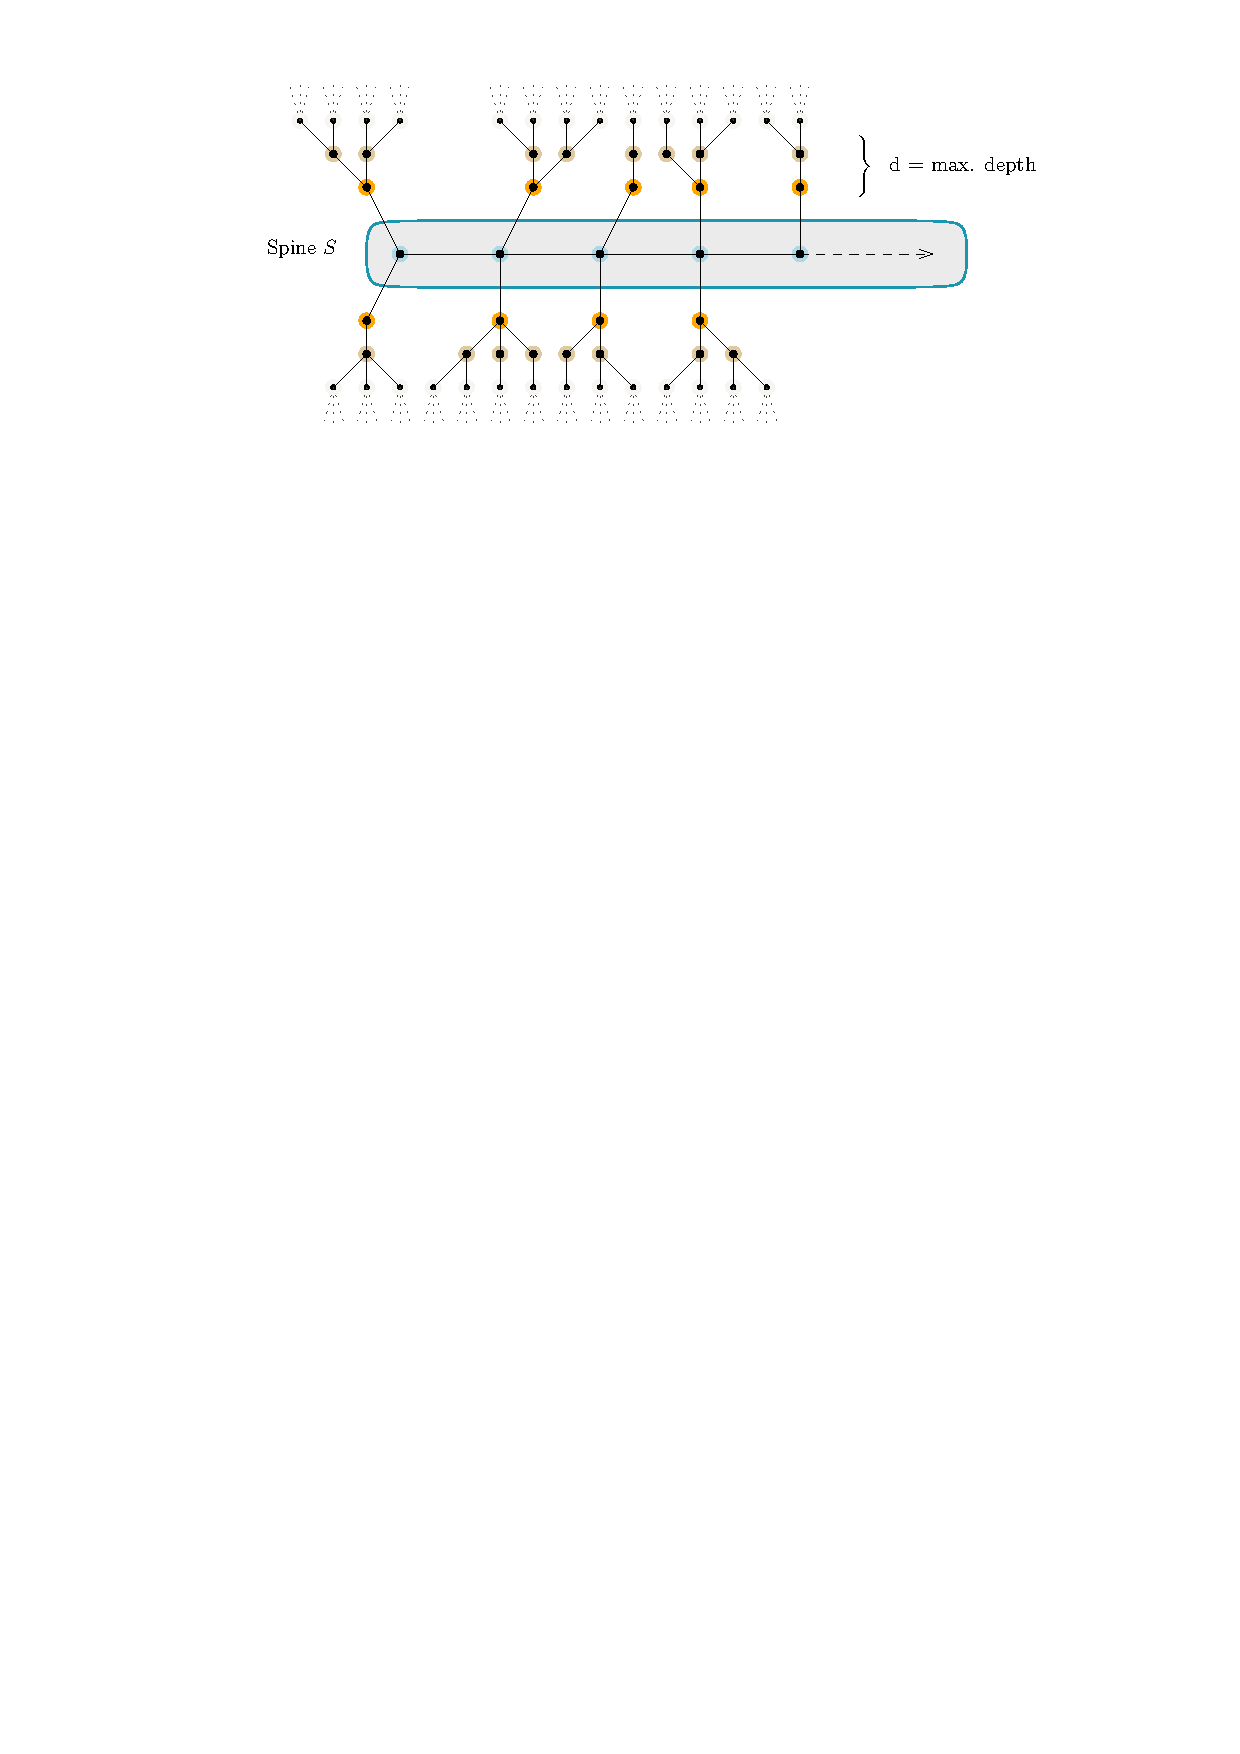
\includegraphics{graphics/ch2_spinedgraph.pdf}
    \caption{A spined graph consists of a string of vertices identified as the \emph{spine}, here marked in blue. Connected to the spine vertices, we find the subtrees rooted in the orange vertices. With unbounded depth and unbounded spine length, spined graphs are little more than trees. However, by bounding $d$ by a constant, we treat ourselves to a new class of graph, simpler than the general tree.}
    \label{fig:ch2_spinedgraph}
\end{figure}

A \emph{caterpillar} is a spined graph $(\Spines \cup \Leaves, E)$ with depth $d=1$, where $\Leaves$ is the set of \emph{leaves}. $\Spines$ and $\Leaves$ are disjoint sets. Every leaf $l \in \Leaves$ is connected to its parent spine vertex $p(l) \in \Spines$: $(l, p(l)) \in E$.

We are now prepared to introduce the graph class which is the core subject of our examination.

\begin{definition}[Lobster]
A lobster is a spined graph $(\Spines \cup \Branches \cup \Leaves, E)$ with depth $d=2$, where $\Branches$ is the set of \emph{branches} and $\Leaves$ is the set of \emph{leaves}.  $\Spines$, $\Branches$ and $\Leaves$ are mutually disjoint sets.

Every branch $b \in \Branches$ is connected to its parent spine vertex $p(b) \in \Spines$: $(b, p(b)) \in E$. Every leaf $l \in \Leaves$ is connected to its parent branch $p(l) \in \Branches$: $(l, p(l)) \in E$.
\end{definition}

\begin{figure}
    \centering
    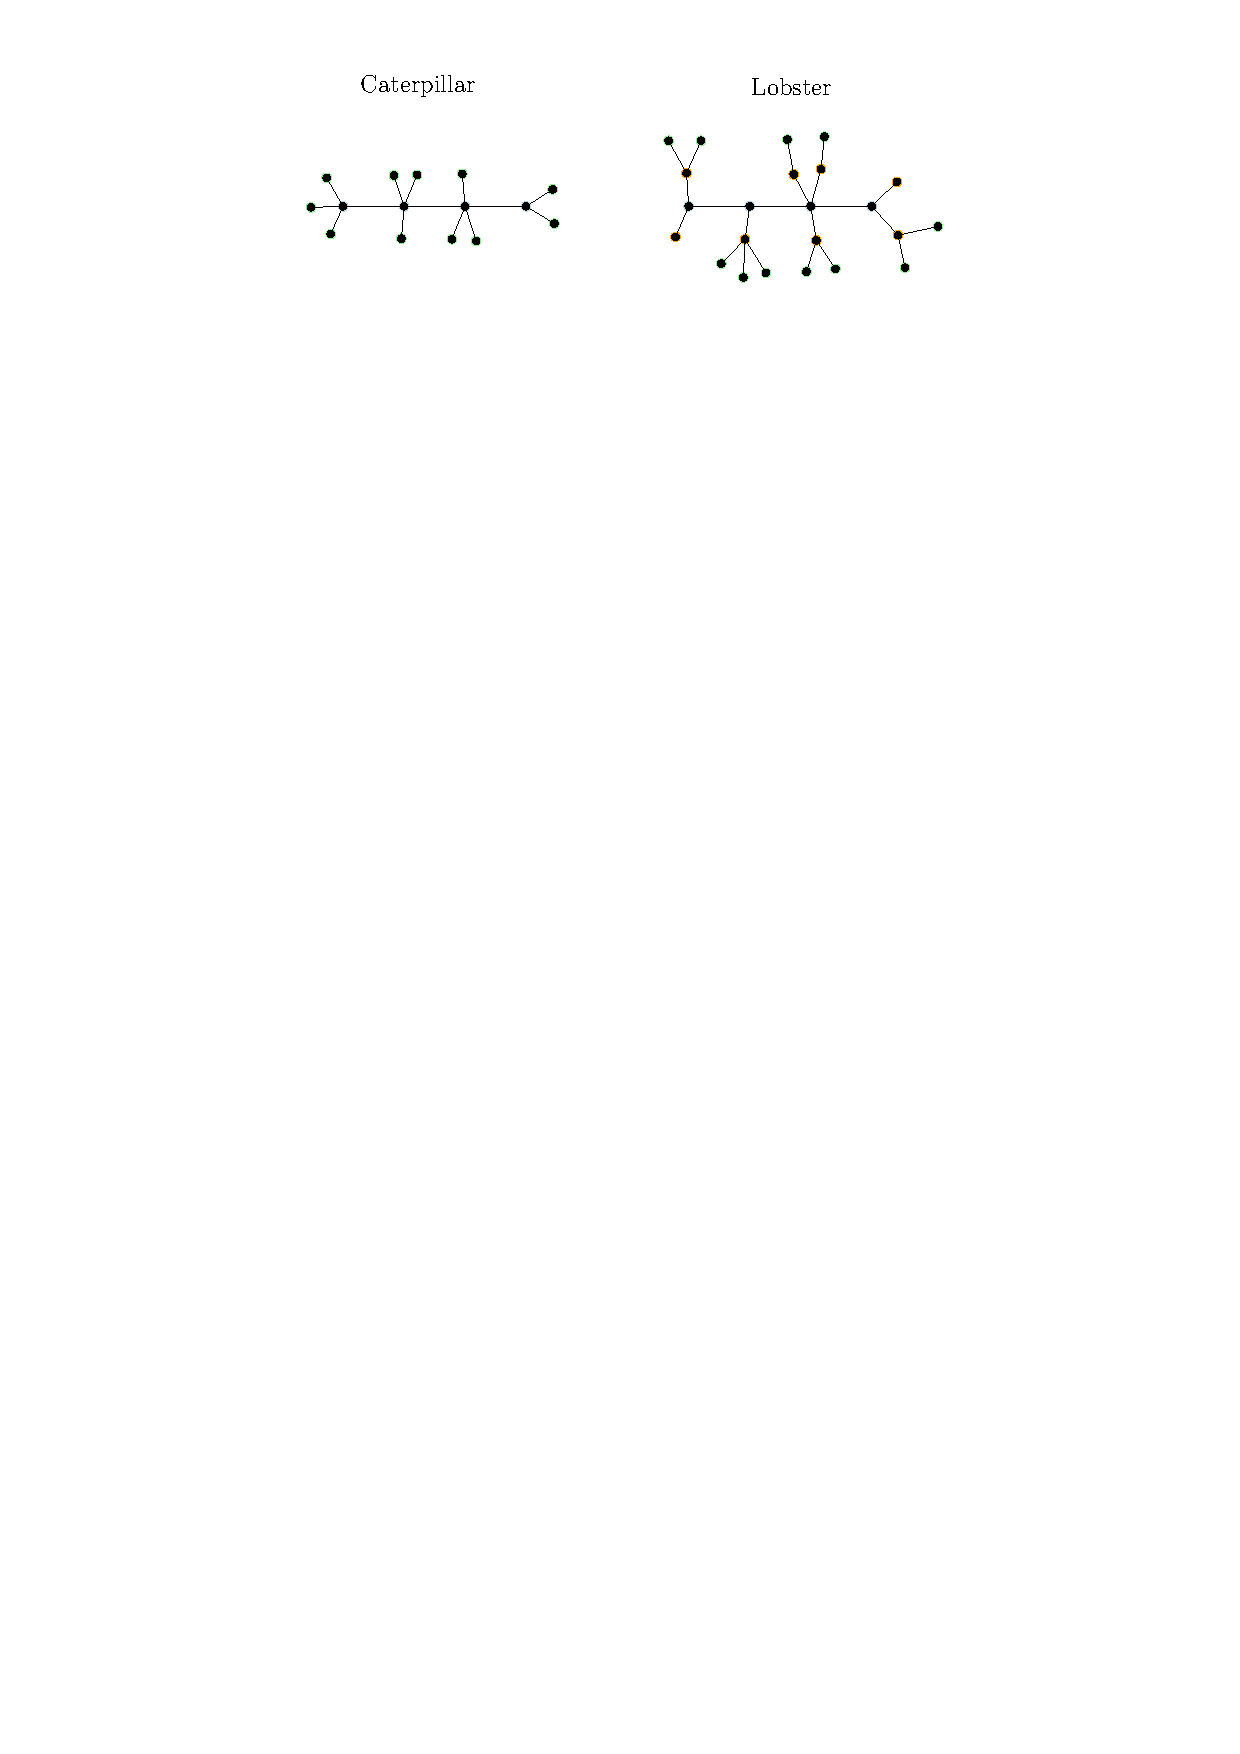
\includegraphics{graphics/ch2_caterpillar_lobster.pdf}
    \caption{The caterpillar and lobster, shown here, are the only kinds of spined graphs which we explore in this thesis.}
    \label{fig:ch2_caterpillar_lobster}
\end{figure}

\section{Representations}

A \emph{combinatorial embedding} (or just \emph{embedding}) of a graph in the plane encodes the topological properties of the graph. For each vertex, the embedding defines the clockwise-ordered arrangement of its neighbors. The embedding is independent of any specific planar coordinates for vertices and edges, but every drawing of a planar graph induces an embedding.

In this thesis, we define the \emph{embedding function} $d$ over $G$ as a bijection $d: V \mapsto \R^2$, which maps vertices to coordinates in the plane. In the common node-link diagram representation, we would draw straight lines to represent the edges. The notation $d$ is short for ``disk'' due to the graph representations below for which we use it.

\soeren[inline]{You define Embedding. Maybe it is helpful to define drawing as the mapping of vertices and edges into the plane and then define the concept of a combinatorial embedding, uniquely defined by such a drawing. Then you can say that in contrast to the usual definition of a drawing, you want to represent graphs differently as unit disk representations, but you have the concept of an embedding, and you can say that a unit disk representation \emph{induces} an embedding by using the centerpoint straight line connections to obtain a drawing and the embedding of that drawing, is also the embedding of the unit disk representation.}
\peter[inline]{I defined it somewhat, but suspect that it needs additional review.}

The \emph{Euclidean norm} $||v||, v = (v_x, v_y)$, is the straight-line length of the vector $v$. $||v|| = \sqrt{v_x^2 + v_y^2}$. $||v_1 - v_2||$ is the distance between the points $v_1$ and $v_2$.

The most common notions of graph drawings represent vertices as points. Numerous alternative representations exist. Drawings in which vertices are represented as disks are of particular interest to us.

\begin{definition}[Disk Contact Representation]
\label{def:ch2_DCR}
Let $G = (V, E)$ be a graph and $d$ be an embedding function over $G$. Further let $w: V \mapsto \mathbb R$ be a \emph{weight function} for the vertices of $G$ such that

\begin{align*}
\lVert d(v_1) - d(v_2) \rVert &= \frac12(w(v_1) + w(v_2)) &\text{ if } (v_1, v_2) \in E \text{ and} \\ \lVert d(v_1) - d(v_2) \rVert &> \frac12(w(v_1) + w(v_2)) &\text{ otherwise.}
\end{align*}

Then $D = (d, w)$ constitutes a \emph{disk contact representation} of $G$.
\end{definition}

\begin{definition}[Weak Disk Contact Representation]
\label{def:ch2_WDCR}
Let $G = (V, E)$ be a graph, $d$ be an embedding function over $G$ and $w$ be a weight function for $V$ such that

\begin{align*}
\lVert d(v_1) - d(v_2) \rVert &= \frac12(w(v_1) + w(v_2)) &\text{ if } (v_1, v_2) \in E \text{ and} \\ \lVert d(v_1) - d(v_2) \rVert &\ge \frac12(w(v_1) + w(v_2)) &\text{ otherwise.}
\end{align*}

Then $D = (d, w)$ constitutes a \emph{weak disk contact representation} of $G$.
\end{definition}

When we want to explicitly refer to the contact notion from Definition~\ref{def:ch2_DCR}, in contrast to the ``weak'' contact from Definition~\ref{def:ch2_WDCR}, we call it ``strict'' or ``proper'' contact. In the rest of this thesis, we mainly concern ourselves with weak contact. Thus, the weak contact notion is assumed as the default in every context from now on unless explicitly specified otherwise. Regardless, the further definitions involving disk contact can be used both with weak and strict notions of contact.

$G$ is a \emph{disk contact graph} if it admits a disk contact representation. A disk contact graph can be drawn by drawing for each vertex $v$ a disk centered at $d(v)$ with diameter $w(v)$. Such graphs are also called ``coin graphs'' in literature. The disk of $v$ precisely touches the disks of neighbouring vertices. Under strict contact, it does not touch any other disks. Under the weak contact notion, disks may touch even if there is no edge between them. In a drawing using disks, there are no curves to represent the edges beyond the disks being in contact or not. Note that every strict disk contact graph is also a weak disk contact graph.

\soeren{I would state this before the definition of the weak unit disk graphs and remove unnecessary words. 'The famous circle packing theorem establishes an equivalence between disk contact representations and planar graphs.' Citation should be in the statement. I added it here as an example. Old citation should be removed.}
\peter{Moved before unit disks. Good enough?}

The famous \emph{circle packing theorem}~\cite{Koebe1936} states that every planar graph admits a (strict) disk contact representation.

Let $G = (\Spines \cup \mathcal T, E), \Spines = \{ s_1, \ldots, s_n \}$ be a spined graph and $D$ be a disk contact representation. $D$ is \emph{x-monotone} if $\forall i > 1: d_x(s_{i+1}) > d_x(s_i),$ where $d_x(v)$ is the x-component of the embedded coordinate of $v$. Informally, the spine ``goes from left to right''.

If it holds for the weight function $w$ of a disk contact representation of $G = (V, E)$ that $\forall v\in V: w(v) = 1$, then we call it a \emph{unit disk contact representation}, shortening ``unit disk contact'' to UDC for readability. $G$ is a UDC graph or UDCG.

Let $D = (d, w)$ be a weak disk contact representation in which $d$ maps all vertices to points from the set $\{ (x + \frac y2, \frac{\sqrt3}2 y) \mid x, y \in \mathbb Z \}$. This set describes the intersection points of a \emph{triangular grid} in the plane, and we call $D$ a \emph{tri-grid representation}. Every such grid point $\coord$ has a \emph{neighborhood}
\begin{align*}\Gamma(\coord) = \Bigg\{ &\coord + (-1, 0); \coord + \left(-\frac12, \frac{\sqrt3}2\right); \coord + \left(\frac12, \frac{\sqrt3}2\right);\\
&\coord + (1, 0); \coord + \left(\frac12, -\frac{\sqrt3}2\right); \coord + \left(-\frac12, -\frac{\sqrt3}2\right) \Bigg\}.\end{align*}
The more restricted \emph{x-monotone neighborhood}
\begin{align*}\Gamma^{x+}(\coord) = \left\{ \coord + \left(\frac12, \frac{\sqrt3}2\right); \coord + (1, 0); \coord + \left(\frac12, -\frac{\sqrt3}2\right) \right\}\end{align*}
includes only those neighbors with a larger x-coordinate than $\coord$.

The triangular grid lends itself to UDC representations because the distance between two neighbor coordinates on the triangular grid is exactly $1$. Consequently, unit disks embedded at neighboring tri-grid points are in contact. So, if $G = (V, E)$ is a disk contact graph, $D = (d, w)$ is a UDC representation, $v \in V, \coord = d(v)$ and $(v, u) \in E$, then $d(u) \in \Gamma(\coord)$.

\section{Problems}

A \emph{recognition problem} is a computational problem in which the goal is to find an algorithm which decides, for a given input from a larger domain, whether that input belongs to a certain smaller class or set in the domain. We say that the algorithm \emph{recognizes} the set.

The broadest problem that we are interested in discussing here is, in the following two variants:

\begin{problem}[Strict UDC Recognition]
Given a graph $G$, does $G$ admit a strict UDC representation?
\label{prob:strict-udc}
\end{problem}

\begin{problem}[Weak UDC Recognition]
Given a graph $G$, does $G$ admit a weak UDC representation?
\label{prob:weak-udc}
\end{problem}

These problems are successors to the original disk contact problem, answered by the above mentioned circle packing theorem. Now restricted to unit size disks, solutions to these problems already exist for the restricted graph class of caterpillars~\cite{Klemz2015}~\cite{Cleve2020}, to be reviewed in Chapter~\ref{chp:related-work}.

As promised in the introduction, we now tie into current research by focusing our attention on the subclass of lobsters. Under the current state of knowledge, we have no algorithm to answer these problems in polynomial time. We can however make some concessions in the form of assumptions to pull the problem into our analytic reach~\cite{Bhore2021}.

\begin{problem}[Tri-Grid X-Monotone UDC Recognition for Lobsters]
Given a lobster $G$, does $G$ admit an x-monotone UDC representation on the triangular grid?
\label{prob:weak-udc-lobster}
\end{problem}
\soeren[inline]{I would call this the Weak UDCG Recognition Problem for Lobsters. Second I think you can define a problem environment as a normal theorem environmant. This looks slightly out of place. I also think this should be the last thing in the preliminaries, where you first introduce what a recognition problem is, then specify the recognition problem for weak trigrid UDCG (which should be defined as graphs taht admit a weak UDCR on a trigrid) and in particular for lobsters. Only the most specific variant of that should be in the problem environment.}
\peter[inline]{problem is now a theorem. weak is default.}

Unit disks on the triangular grid are packed decently dense. Tighter packing configurations exist, but because this grid is nice and regular and our relevant spine graphs---lobsters---only extend up to two neighbors from the spine, we can assume that the slightly sub-optimal density of our chosen packing configuration does not impact our results compared to the arbitrary configuration. In other words, we assume that a given lobster $G$ admits a tri-grid UDC representation if it admits any UDC representation. This assumption also motivates our use of the weak contact notion, which ``unlocks'' the tri-grid configuration for easier analysis.

Likewise, we allow ourselves the restriction to x-monotone solutions based on the unproven assumption that a given lobster $G$ admits an x-monotone UDC representation if it admits any UDC representation. As there is no combinatorial embedding prescribed for $G$, no branch necessarily has to be above or below the spine. Yet, to refute our x-monotonicity assumption, a counter-example lobster would have to have some configuration of branches and leaves such that all its possible UDC representations enforce either an acute ($60^\circ$) ``bend'' in the spine, or two consecutive obtuse ($120^\circ$) bends in the same direction. By superficial experimentation, it appears that such configurations do not occur.

With the subject problem properly outlined, we explore the current state of research on the following questions:

\begin{enumerate}
    \item[Question 1:] Can we decide the weak UDC recognition problem for lobsters of size $n$ in time $O(n)$?
    \item[Question 2:] Can we decide the tri-grid x-monotone UDC recognition problem for lobsters of size $n$ in time $O(n)$?
\end{enumerate}

\begin{figure}
    \centering
    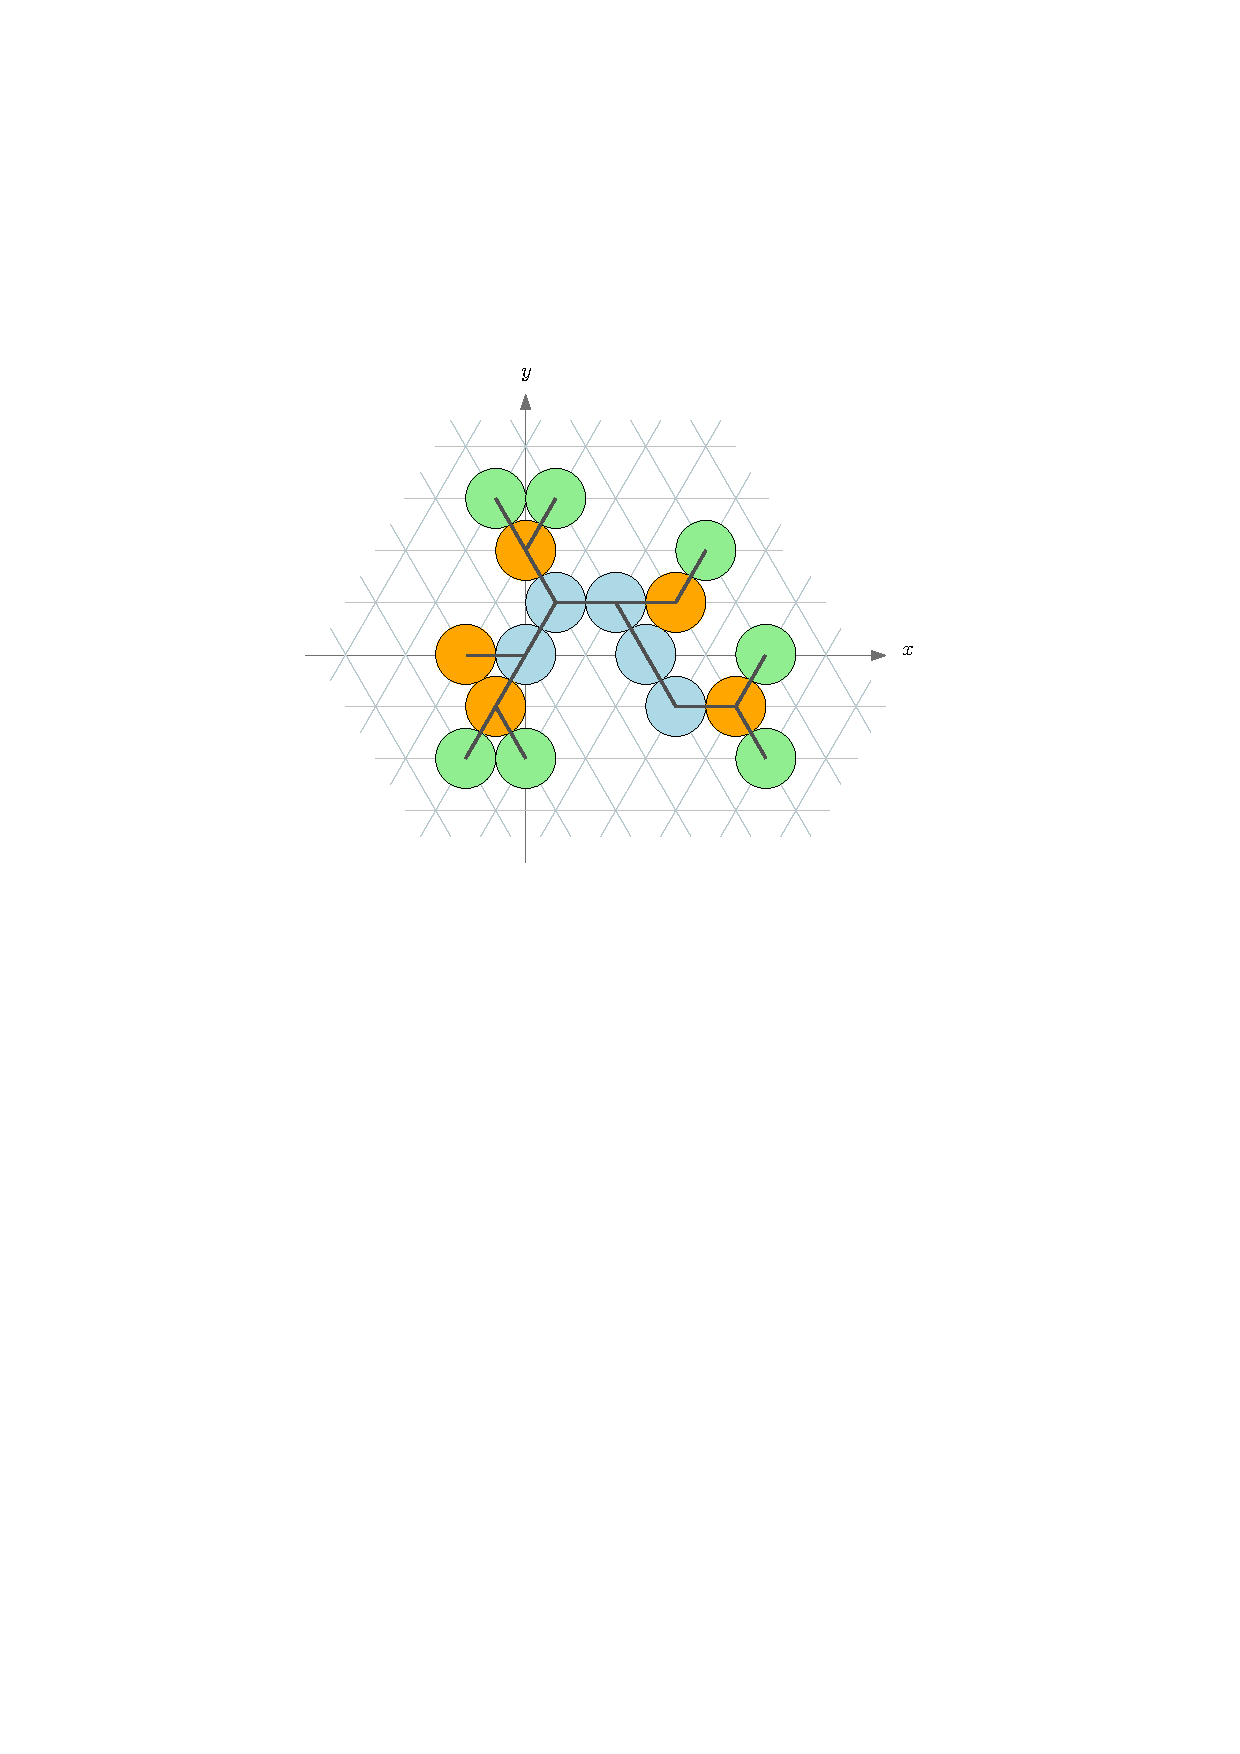
\includegraphics{graphics/ch2_tri-grid_x-monotone.pdf}
    \caption{A tri-grid x-monotone UDC representation of a lobster. The spine, although it bends twice, is embedded on strictly increasing x-coordinates.}
    \label{fig:ch2_tri-grid_x-monotone}
\end{figure}

\soeren[inline]{Everything below here needs to be restructured. The Conjectures shouldn't be in this preliminaries section. Or at least I would change the way things are introduced here. So before stating the conjecture, first define the trigrid representation on its own, as well as the concept of an $x$-monotone representation. The idea is the you defined these terms before you use them in the conjectures. Then I would not formulate them as conjectures at all, since a conjecture usually means 'We looked into this, we have an inclination but at the end of this publiucation we can not prove it.' Here I think 'Question' would be the right term. HERE WE SHOULD DISCUSS HOW TO STRUCTURE EVERYTHIng. But that seems easier in person}
\peter[inline]{Restructured preliminaries ready for next review.}

\soeren[inline]{Reihenfolge: Spined graphs, then DG, define UDG and weak DG as special cases. Define recognition question for UDG and weak UDG. Then define trigrid UDR (including neighborhood) and what a monotone UDR (including monotone neighborhood) is. Then define problem 3 as weak trigrid monotone UDG recognition. Finally state that it is unclear if every spined graph that admits a wUDR also admits a monotone one on the grid. Be specific about caterpillars and lobsters in related work.}
\peter[inline]{about right}
